
%%%%%%%%%%%%%%%%%%%%%%% file typeinst.tex %%%%%%%%%%%%%%%%%%%%%%%%%
%
% This is the LaTeX source for the instructions to authors using
% the LaTeX document class 'llncs.cls' for contributions to
% the Lecture Notes in Computer Sciences series.
% http://www.springer.com/lncs       Springer Heidelberg 2006/05/04
%
% It may be used as a template for your own input - copy it
% to a new file with a new name and use it as the basis
% for your article.
%
% NB: the document class 'llncs' has its own and detailed documentation, see
% ftp://ftp.springer.de/data/pubftp/pub/tex/latex/llncs/latex2e/llncsdoc.pdf
%
%%%%%%%%%%%%%%%%%%%%%%%%%%%%%%%%%%%%%%%%%%%%%%%%%%%%%%%%%%%%%%%%%%%


\documentclass[runningheads,a4paper]{llncs}
\usepackage{graphicx}
\usepackage{url}
\usepackage[listings]{tcolorbox}
\usepackage{amssymb}
\usepackage{pifont}

\newcommand{\critics}{{\small{\sc{Critics}}}}
\newcommand{\phabricator}{{\small{\sc{Phabricator}}}}
\newcommand{\gerrit}{{\small{\sc{Gerrit}}}}
\newcommand{\codeflow}{{\small{\sc{CodeFlow}}}}
\newcommand{\collaborator}{{\small{\sc{Collaborator}}}}
\newcommand{\clusterchanges}{{\small{\sc{ClusterChanges}}}}
\newcommand{\delCode}{\textcolor{black}}
\newcommand{\addCode}{\textcolor{black}}
\newcommand{\ttt}[1]{\tt\small{#1}}


% -----------------------------------------------------------------
% color
% -----------------------------------------------------------------
\definecolor{javared}{rgb}{0.6,0,0} % for strings
\definecolor{javagreen}{rgb}{0.25,0.5,0.35} % comments
\definecolor{javapurple}{rgb}{0.5,0,0.35} % keywords
\definecolor{javadocblue}{rgb}{0.25,0.35,0.75} % javadoc

% ===============================================
% MyJavaSmallStyle
% ===============================================
\lstdefinestyle{MyJavaSmallStyle} {
  language=Java,
  frame=none,
  xleftmargin=15pt, 
  stepnumber=1, 
  numbers=left, 
  numbersep=5pt,
  numberstyle=\tiny\color[gray]{0.777}, 
  belowcaptionskip=\bigskipamount,
  captionpos=b, 
  escapeinside={*'}{'*},
  tabsize=5,
  emphstyle={\bf},
  basicstyle=\scriptsize\ttfamily,
  keywordstyle=\color{javapurple}\bfseries,
  stringstyle=\color{javared},
  commentstyle=\color{javagreen},
  morecomment=[s][\color{javadocblue}]{/**}{*/},
  showspaces=false,
  columns=flexible,
  showstringspaces=false,
  morecomment=[l]{//},
  tabsize=2,
  morekeywords={, Package,Invariant,Class,Method,Field,Where,in,Assert,ToLc,Split,Msg,Immutable,<<<,eq,neq,not,has,Assert,AssertExists,Attribute,Uc,Lc,},
  breaklines=true
}

\usepackage{amssymb}
\setcounter{tocdepth}{3}
\usepackage{graphicx}

\usepackage{url}

\newcommand{\keywords}[1]{\par\addvspace\baselineskip

\noindent\keywordname\enspace\ignorespaces#1}
\newcommand{\codefont}[1]{\footnotesize{\texttt{#1}}\normalsize}


\begin{document}

\mainmatter  % start of an individual contribution

% first the title is needed
\title{Software Evolution} 

% a short form should be given in case it is too long for the running head
\titlerunning{Lecture Notes in Computer Science: Authors' Instructions}

% the name(s) of the author(s) follow(s) next
%
% NB: Chinese authors should write their first names(s) in front of
% their surnames. This ensures that the names appear correctly in
% the running heads and the author index.
%
\author{Na Meng, Tianyi Zhang, Miryung Kim} 

\institute{Virginia Tech and University of California, Los Angeles} 


\toctitle{Handbook on Software Engineering} 
\tocauthor{Na Meng, Tianyi Zhang and Miryung Kim}
\maketitle


\begin{abstract}
	\todo{Miryung is in charge.} 
\end{abstract}


\section{Introduction}
\todo{2 page-Miryung is in charge}
- explain the definition of software evolution (cite: belady and lehman, etc)
%L.A. Belady and M.M. Lehman, a Model of Large Program Development,o IBM Systems J., vol. 15, no. 1, pp. 225±252, 1976.
\cite{Belady1976:ModelEvolution} 
% follow up work by Yuen 
@inproceedings{ChongHokYuen1986:EAS,
 author = {Chong Hok Yuen, C S},
 title = {An Empirical Approach to the Study of Errors in Large Software Under Maintenance},
 booktitle = {The Institute of Electrical and Electronics Engineers, Inc on Conference on Software Maintenance--1985},
 year = {1985},
 isbn = {0-8186-0648-7},
 location = {Washington, D.C, USA},
 pages = {96--105},
 numpages = {10},
 url = {http://dl.acm.org/citation.cfm?id=20924.20936},
 acmid = {20936},
 publisher = {IEEE Press},
 address = {Piscataway, NJ, USA},
} 

% some overview materials can be drawn from then introduction of kemerer paper. 
- describe why this chapter focus on code changes, rather than other types of artefacts such as requirements, specifications, design documents, etc. 
- argue why software evolution is important (cite: code decay, eick et al.) 
\cite{Eick2001:CodeDecay}

\section{Concepts and Principles}

\todo{4 page-Na is in charge} 
- explain a broad category of changes: corrective, adaptive, and perfective changes (cite kemerer and slaugher)  

E.B. Swanson, The Dimensions of Maintenance, Proc. Second Int'l Conf. Software Eng., 1976.

@inproceedings{Swanson1976:Dimension, 
 author = {Swanson, E. Burton},
 title = {The Dimensions of Maintenance},
 booktitle = {Proceedings of the 2Nd International Conference on Software Engineering},
 series = {ICSE '76},
 year = {1976},
 location = {San Francisco, California, USA},
 pages = {492--497},
 numpages = {6},
 url = {http://dl.acm.org/citation.cfm?id=800253.807723},
 acmid = {807723},
 publisher = {IEEE Computer Society Press},
 address = {Los Alamitos, CA, USA},
 keywords = {Performance measurement, Software maintenance},
} 

E.B. Swanson and C.M. Beath, Departmentalization in Software Development and Maintenance,o Comm. ACM, vol. 33, no. 6, pp. 658-667, 1990.
@article{Swanson1990:Departmentalization, 
 author = {Swanson, E. Burton and Beath, Cynthia Mathis},
 title = {Departmentalization in Software Development and Maintenance},
 journal = {Commun. ACM},
 issue_date = {June 1990},
 volume = {33},
 number = {6},
 month = jun,
 year = {1990},
 issn = {0001-0782},
 pages = {658--667},
 numpages = {10},
 url = {http://doi.acm.org/10.1145/78973.78976},
 doi = {10.1145/78973.78976},
 acmid = {78976},
 publisher = {ACM},
 address = {New York, NY, USA},
 keywords = {development, maintenance, management, organizational forms},
} 

- include a diagram about the process of software evolution with focus on changes: (A) applying program changes (B) inspecting program changes, and (C) debugging and testing program changes to overview the rest of sections.  

- introduce topics under each of the three perspectives on program changes. 

\section{An Organized Tour of Seminal Papers: I. Applying Program Changes}

\todo{make the following text a little bit less like compiler optimization and small program transformation. start from three broad categories of changes.}
Program transformation is the process to transform a program to another program. A typical example is compilers. As shown in Figure~\ref{fig:javacompilation}, a Java compiler transforms Java source code into Java bytecode, an intermediate representation of the program. The bytecode can be either interpreted by a bytecode interpreter to directly execute on Java Virtual Machine (JVM), or further transformed by a Just-in-Time (JIT) compiler to machine code for faster execution.

\todo{Miryung to Na, could you please update the figure so that we can discuss program transformations in a broader sense?} 
\begin{figure}
\centering
\scalebox{0.4}{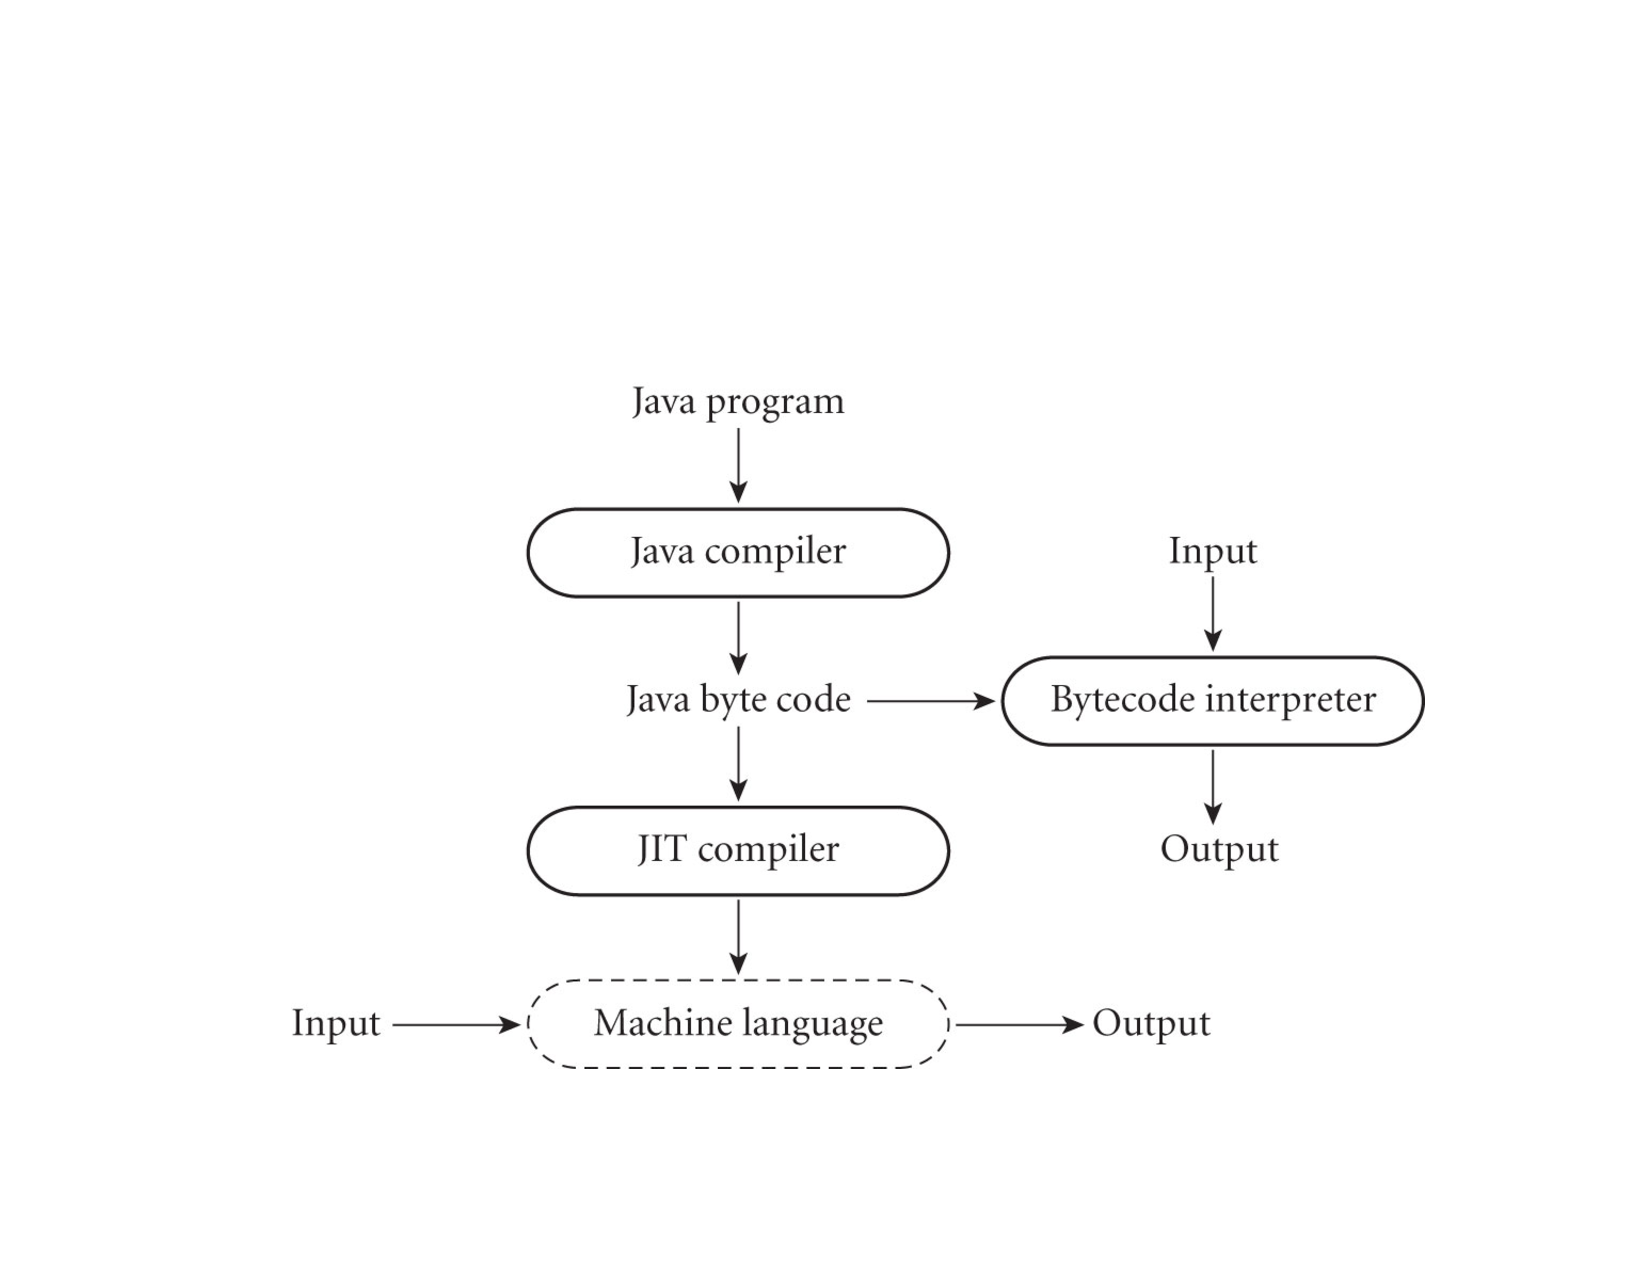
\includegraphics{images/javacompilation.pdf}}
\caption{Java compilation system}
\label{fig:javacompilation}
\end{figure}

\todo{Adapt the following text to meet the new outline / categorization. Also make the text not to just focus on automated transformation, but include other empirical studies on code changes, and how people make such changes manually.} 


Manually transforming programs is tedious and error-prone, because people make mistakes when manipulating code to enforce the explicit or implicit transformation rules.
Various automatic systems have been built to transform programs in a mechanic way. Such systems are built for different purposes. For instance, a source-to-source compiler translates programs from one programming language to another language. Source code generation produces source code based on an ontological model, which defines the types, properties, and interrelationships of entities. 
Many systems guarantee that each transformed program is semantically equivalent to the original program, while other systems do not preserve such semantic equivalence while transforming code. In this section, we will first overview various methods, techniques, and tools to automate source-to-source program transformation (Section~\ref{sec:automated}), and then especially discuss refactoring---one kind of semantic-preserving transformation (Section~\ref{sec:refactoring}), and systematic editing---one kind of transformation that does not preserve semantics (Section~\ref{sec:sysedit}).

\subsection{Perfective Changes} 
\todo{Start from Bill Griswold and Okdype, Ralph Johnson} 

\todo{page length: 1.5 page, overview from Okdype thesis. add an example refactoring}. 
% http://www.laputan.org/pub/papers/opdyke-thesis.pdf 
% formalization of 4 refactorings in terms of pre-condition, post-condition and transformation 
% include one example, rename refactoring. 
@phdthesis{Opdyke:1992:ROF:169783,
 author = {Opdyke, William F.},
 title = {Refactoring Object-oriented Frameworks},
 year = {1992},
 note = {UMI Order No. GAX93-05645},
 publisher = {University of Illinois at Urbana-Champaign},
 address = {Champaign, IL, USA},
} 
\todo{page length: 0.5 page, discuss the work by Griswold:1992}
% an earliest form of IDE-like automated refactoring. Talk about how the formalization of refactoring transforamtions work led to automatedrefactoring. 
@article{Griswold1993:AutomatedRefactoring,
 author = {Griswold, William G. and Notkin, David},
 title = {Automated Assistance for Program Restructuring},
 journal = {ACM Trans. Softw. Eng. Methodol.},
 issue_date = {July 1993},
 volume = {2},
 number = {3},
 month = jul,
 year = {1993},
 issn = {1049-331X},
 pages = {228--269},
 numpages = {42},
 url = {http://doi.acm.org/10.1145/152388.152389},
 doi = {10.1145/152388.152389},
 acmid = {152389},
 publisher = {ACM},
 address = {New York, NY, USA},
 keywords = {CASE, flow analysis, meaning-preserving transformations, software engineering, software evolution, software maintenance, software restructuring, source-level restructuring},
} 

% a survey of software refactoring - Tom Mens
\todo{Miryugn to Na: we should discuss a survey of refactoring papers by Mens} 
@article{Mens2004,
 author = {Mens, Tom and Tourw{\'e}, Tom},
 title = {A Survey of Software Refactoring},
 journal = {IEEE Trans. Softw. Eng.},
 issue_date = {February 2004},
 volume = {30},
 number = {2},
 month = feb,
 year = {2004},
 issn = {0098-5589},
 pages = {126--139},
 numpages = {14},
 url = {http://dx.doi.org/10.1109/TSE.2004.1265817},
 doi = {10.1109/TSE.2004.1265817},
 acmid = {972286},
 publisher = {IEEE Press},
 address = {Piscataway, NJ, USA},
 keywords = {Coding tools and techniques, programming environments/construction tools, restructuring, reverse engineering, and reengineering.},
} 

\paragraph{Refactoring Practices} 
\todo{1 page: Write the following paragraph more broadly. refactoring is a special category of automated transformation: refactoring practices (kim et al., emerson murphy hill, ralph johnson) } 

@inproceedings{Kim2012:FieldStudy, 
 author = {Kim, Miryung and Zimmermann, Thomas and Nagappan, Nachiappan},
 title = {A Field Study of Refactoring Challenges and Benefits},
 booktitle = {Proceedings of the ACM SIGSOFT 20th International Symposium on the Foundations of Software Engineering},
 series = {FSE '12},
 year = {2012},
 isbn = {978-1-4503-1614-9},
 location = {Cary, North Carolina},
 pages = {50:1--50:11},
 articleno = {50},
 numpages = {11},
 url = {http://doi.acm.org/10.1145/2393596.2393655},
 doi = {10.1145/2393596.2393655},
 acmid = {2393655},
 publisher = {ACM},
 address = {New York, NY, USA},
 keywords = {churn, component dependencies, defects, empirical study, refactoring, software evolution},
}

@article{Kim2014:EmpiricalStudy, 
 author = {Kim, Miryung and Zimmermann, Thomas and Nagappan, Nachiappan},
 title = {An Empirical Study of RefactoringChallenges and Benefits at Microsoft},
 journal = {IEEE Trans. Softw. Eng.},
 issue_date = {July 2014},
 volume = {40},
 number = {7},
 month = jul,
 year = {2014},
 issn = {0098-5589},
 pages = {633--649},
 numpages = {17},
 url = {http://dx.doi.org/10.1109/TSE.2014.2318734},
 doi = {10.1109/TSE.2014.2318734},
 acmid = {2693292},
 publisher = {IEEE Press},
 address = {Piscataway, NJ, USA},
} 

%http://ieeexplore.ieee.org/abstract/document/6112738/

@ARTICLE{Murphy-Hill2012:refactor, 
author={E. Murphy-Hill and C. Parnin and A. P. Black}, 
journal={IEEE Transactions on Software Engineering}, 
title={How We Refactor, and How We Know It}, 
year={2012}, 
volume={38}, 
number={1}, 
pages={5-18}, 
keywords={software maintenance;software tools;Eclipse developers;Mylyn developers;randomly sampled code;refactoring tools;research and development;Java;Refactoring;Software tools;Refactoring;floss refactoring;refactoring tools;root-canal refactoring.}, 
doi={10.1109/TSE.2011.41}, 
ISSN={0098-5589}, 
month={Jan},}

@INPROCEEDINGS{Vailian2012:misuse, 
author={M. Vakilian and N. Chen and S. Negara and B. A. Rajkumar and B. P. Bailey and R. E. Johnson}, 
booktitle={2012 34th International Conference on Software Engineering (ICSE)}, 
title={Use, disuse, and misuse of automated refactorings}, 
year={2012}, 
pages={233-243}, 
keywords={software maintenance;software tools;awareness;behavioral data;interaction data;invocation method;lightweight methods;naming;predictability;predictable automated refactorings;refactoring tools;trust;Context;Educational institutions;Interviews;Programming;Reliability;Software;User interfaces;Human computer interaction;Human factors;Programming environments;Software engineering;Software maintenance;User interfaces}, 
doi={10.1109/ICSE.2012.6227190}, 
ISSN={0270-5257}, 
month={June},}

Code refactoring is the process of restructuring source code without changing its external behaviors. It is usually applied to improve code readability or extensibility, or to reduce code complexity. 
Fowler et al.~defined a catalog of refactorings that developers can apply to improve their codebase in different ways~\cite{1999:RID}, although developers can also define and manually apply their own refactorings. Eclipse IDE also provides tool support to automate some of the refactorings mentioned in Fowler's catalog, such as \emph{Extract Method}, \emph{Pull up Method}, and \emph{Move Field}. Researchers proposed various approaches to automate refactoring or to complete the refactoring tasks initiated by developers~\cite{Griswold:1992,Balazinska1999,Dig:2009,Ge:2012,Chen:2013,Lee:2013,Tsantalis2013:icsm,Meng:2015,Kim:2016}.


To ensure the semantic equivalence between programs that are before and after a predefined refactoring program transformation, automated tools always check some pre-conditions before applying the transformation, and may check some post-conditions after the transformation.
In this section, we will explain two refactoring tools with more details: Drag-and-Drop Refactoring (DNDRefactoring)~\cite{Lee:2013} and R3~\cite{Kim:2016}.

\todo{Miryung to Na: DND refactoring does not seem like a seminal paper. Reduce the space allocation of this example section to 1 paragraph after discussing some seminal papers first.} 
\paragraph{Drag-and-Drop Refactoring.} Prior research identified at least three dominant usability problems when using automated refactoring tools~\cite{OConnor:2005,Mealy:2007,Parnin:2008,Murphy-Hill:2008,Murphy-Hill:2011,Vakilian:2012}. First, programmers have trouble identifying opportunities for using the tools. Second, programmers have difficulty invoking the right refactoring from a lengthy menu of available refactorings. Third, programmers find it complicated to properly configure refactoring dialogs. DNDRefactoring was proposed to facilitate automated refactoring by allowing programmers to apply refactorings through direct manipulation on program elements, including variables, expressions, statements, and methods, in the IDE. In this way, developers do not need menus or dialogs to specify what refactoring to apply or how to apply those refactorings. Instead, DNDRefactoring can automatically infer such information by monitoring the selection and drag-and-drop operations of developers.

Figure~\ref{fig:dnd} presents two scenarios where DNDRefactoring automates refactorings based on the gestures of developers in Eclipse IDE. As shown in Figure~\ref{fig:dnd} (a), when developers select a code snippet in an existing method \codefont{bar(...)}, and then drag-and-drop the snippet to a location outside \codefont{bar(...)}, DNDRefactoring automates the \emph{Extract Method} refactoring by creating a new method \codefont{extracted(...)}, which takes in one parameter: \codefont{name}. In this process, no menu or configuration dialog is needed, because the tool can infer developers' refactoring intent, and decide all detailed information required for the refactoring, such as the method name, the method body, and the code location where to place the new method. Figure~\ref{fig:dnd} (b) shows another scenario. When developers manually select the \codefont{InnerClass}, a class declared inside another class \codefont{OuterClass}, and then drag-and-drop the class to a package \codefont{pkg}, DNDRefactoring infers that developers want to extract the type and create a new Java file. Therefore, it generates a Java file InnerClass.java to hold all implementation of \codefont{InnerClass}.

\begin{figure}
\centering
\scalebox{0.5}{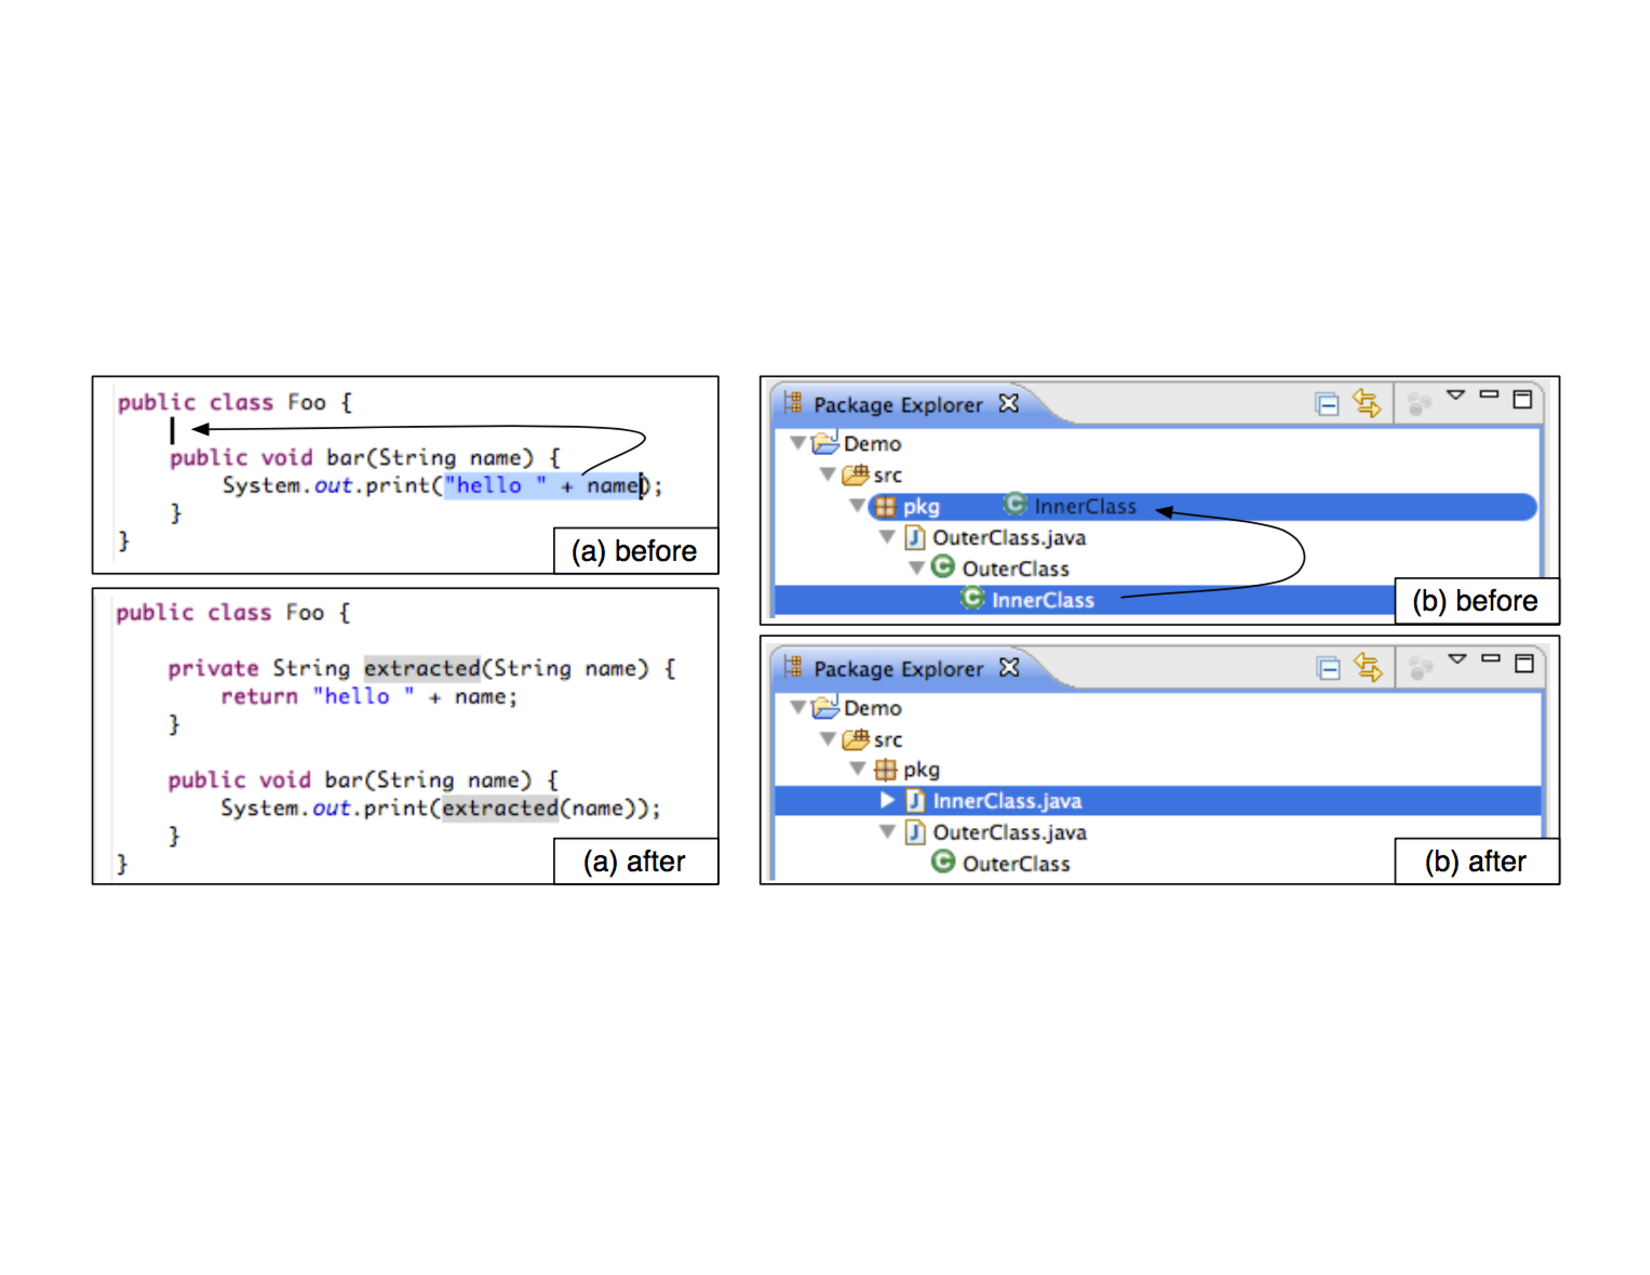
\includegraphics{images/DNDRefactoring.pdf}}
\caption{DNDRefactoring: Drag-and-drop gestures in (a) Java editor for Extract Method refactoring, and (b) Package Explorer for Extract Type to New File refactoring~\cite{Lee:2013}.}
\label{fig:dnd}
\end{figure}

@inproceedings{Lee013:DNDRefactoring, 
 author = {Lee, Yun Young and Chen, Nicholas and Johnson, Ralph E.},
 title = {Drag-and-drop Refactoring: Intuitive and Efficient Program Transformation},
 booktitle = {Proceedings of the 2013 International Conference on Software Engineering},
 series = {ICSE '13},
 year = {2013},
 isbn = {978-1-4673-3076-3},
 location = {San Francisco, CA, USA},
 pages = {23--32},
 numpages = {10},
 url = {http://dl.acm.org/citation.cfm?id=2486788.2486792},
 acmid = {2486792},
 publisher = {IEEE Press},
 address = {Piscataway, NJ, USA},
} 

Although DNDRefactoring demonstrated effectiveness in simplifying the application of automated refactorings, it still suffers from several limitations. First, not every refactoring can be conducted in a drag-and-drop manner. DNDRefactoring effectively supports move- and extract-based refactorings, but does not support \emph{Rename} refactoring. If developers want to rename a variable or a class, they cannot express that intent via selecting some text and moving it around with the cursor. Second, even for move- or extract- based refactorings, DNDRefactoring mainly works when the drag source and drop target elements are shown in the same screen. It does not work when these elements are located too far away to be presented in the same visual editor simultaneously. Third, DNDRefactoring does not allow users to freely configure refactoring details. For example, when users want to specify a meaningful name of an extracted method, with DNDRefactoring, they have no way to customize the information.

\todo{Miryung to Na. R3 does not seem like a seminal paper. Similarly, you should reduce the space allocation to 1 paragraph} 
@INPROCEEDINGS{Kim2016:R3, 
author={J. Kim and D. Batory and D. Dig and M. Azanza}, 
booktitle={2016 IEEE/ACM 38th International Conference on Software Engineering (ICSE)}, 
title={Improving Refactoring Speed by 10X}, 
year={2016}, 
pages={1145-1156}, 
keywords={Java;software maintenance;AST;Eclipse Java development tools;Gang-of-Four text;IDE;JDT;Java entity declarations;Java refactoring engine;abstract syntax trees;integrated development environment;refactoring script;refactoring sequence;refactoring speed;retrofitting design patterns;Computer bugs;Databases;Engines;Graphical user interfaces;Graphics;Java;Maintenance engineering}, 
doi={10.1145/2884781.2884802}, 
month={May},}
\paragraph{R3.} Compared with DNDRefactoring which improves the usability of Eclipse Refactoring with better UIs, R3 presents an alternative refactoring engine that works 10 times faster than Eclipse Refactoring. Specifically, R3 provides refactoring scripts as short Java methods, which enables users to easily define new refactorings. 
To speed up the application of refactorings, R3 first parses Java sources files, and builds a main-memory, non-persistent database to encode Java entity declarations (e.g., packages, class, methods), their containment relationships, and language features such inheritance and modifiers. By converting program Abstract Syntax Tree (AST) transformations to database queries and manipulations, R3 significantly reduces the runtime overhead of automating refactorings.

\begin{figure}
\centering
\scalebox{0.5}{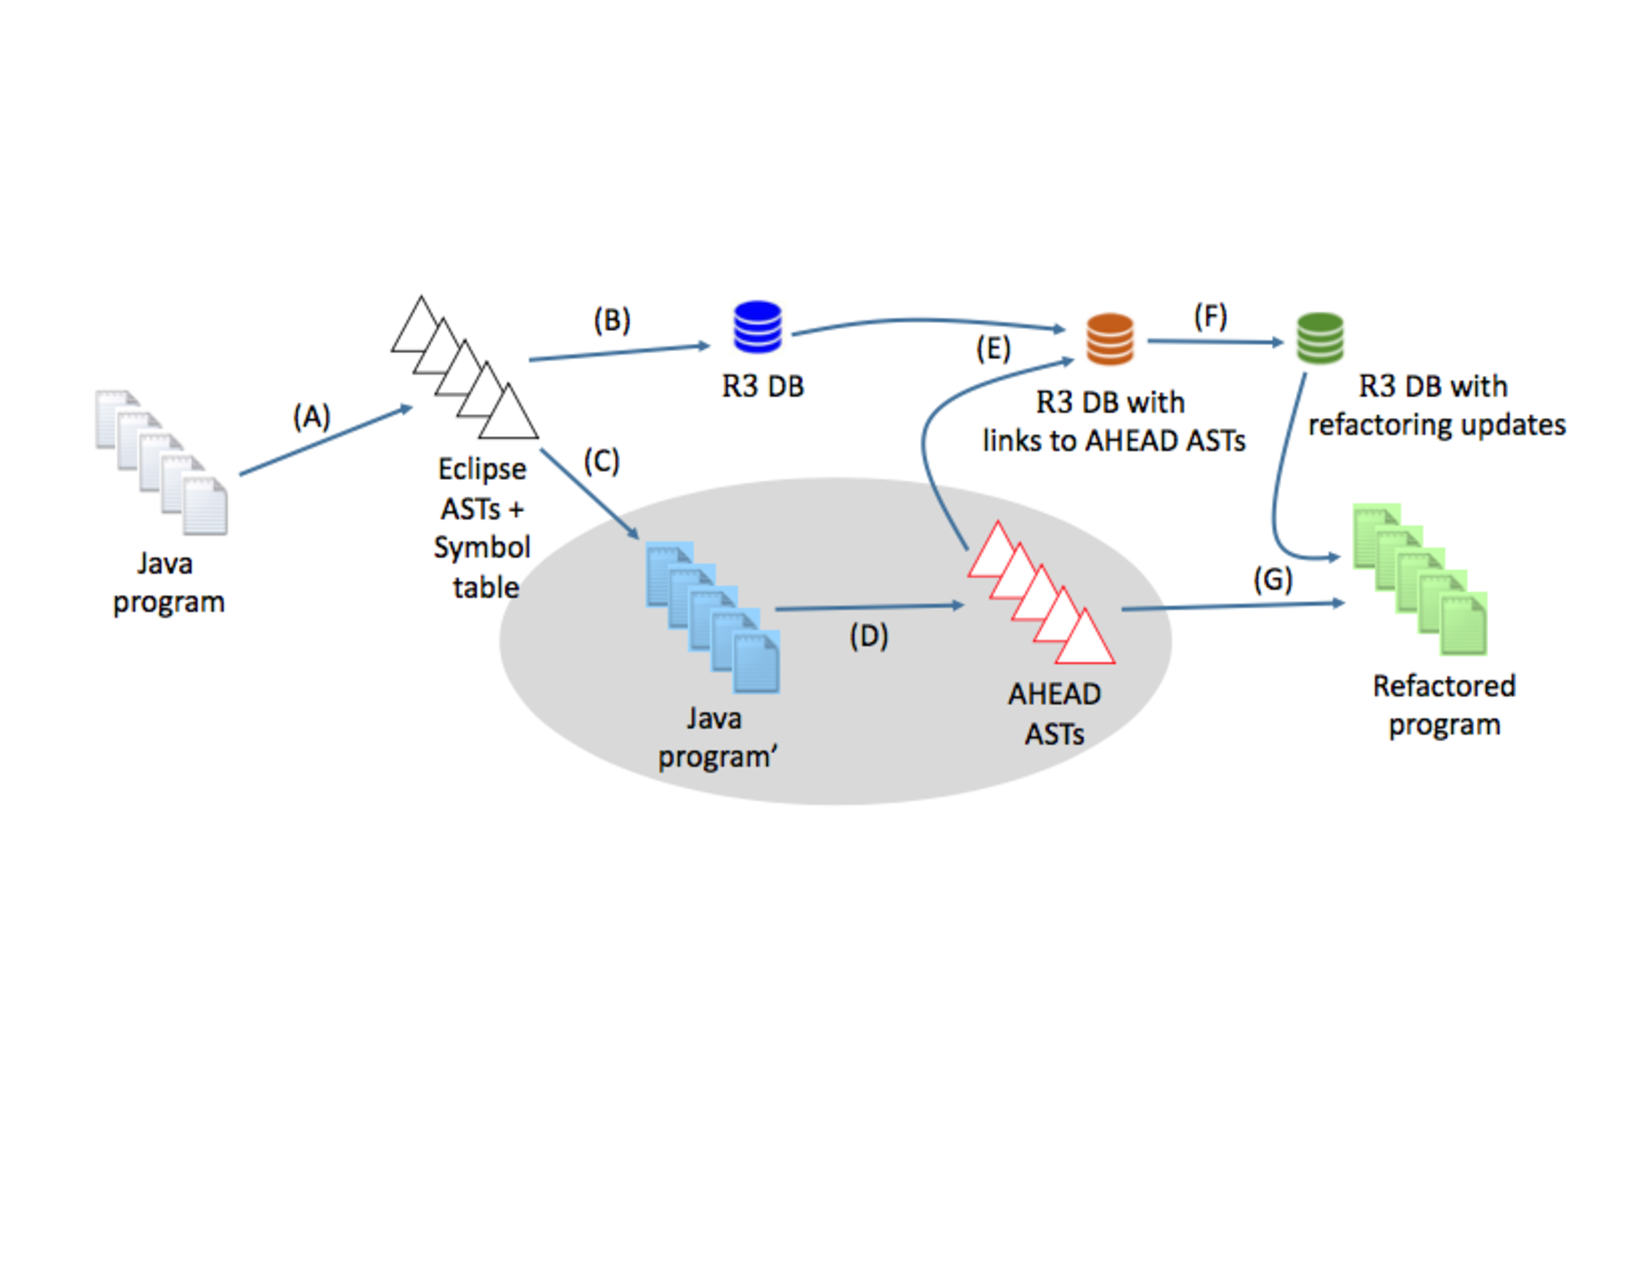
\includegraphics{images/r3overview.pdf}}
\caption{R3 pipeline~\cite{Kim:2016}.}
\label{fig:r3overview}
\end{figure}

Figure~\ref{fig:r3overview} presents the R3 pipeline, which has a series of stages (A)-(G) that map a target Java program (JDT project) on the left to a refactored program on the right. Stage (A) parses a Java program into ASTs with an Eclipse ASTParser. Stage (B) visits each generated AST to gather all Java entity-relevant information, and to save the information in R3 DB. To prepare program refactorings based on R3 DB, stage (C) generalizes the original program by replacing concrete entity information with abstract symbolic names, with each name corresponding to one concrete entity identifier kept in R3 DB. Stage (D) uses AHEAD~\cite{Batory:2003} to further parse the generalized program representation and create AHEAD ASTs. In Stage (E), tuples in R3 DB are doubly-linked to their AHEAD AST nodes, so that each pretty-printer of an AST node can reference the corresponding R3 tuple and vice versa. 

Stage (F) execute R3 refactorings. Unlike classical refactoring engines that modify Abstract Syntax Trees (ASTs), R3 refactorings modify only the database. For instance, if developers want to move a method from one class to another class, R3 does not directly move the method AST. Instead, it simply updates the method's database entry to have the new receiver type. With such information updates to the database, R3 can avoid repetitive AST manipulations. Finally, according to the updated entity information in R3 DB, stage (G) pretty-prints the source code, producing the resulting refactored program.

In addition to converting expensive AST manipulations to cheap database updates, R3 also precomputes the value of many properties of Java entities and saves those values in its database. Since these values can be used int the precondition checks of many refactoring tasks, keeping them in the database can avoid repetitive value computations, which can further reduce runtime overhead. R3 can well handle move- and rename-based refactorings, but does not support extract-based refactorings, because it does not store or modify statement-level or expression-level information in the database.  
\subsection{Corrective Changes} 
	- discuss literature on bug fixes  


\todo{1 page: discuss characteristics of bug fixes from the two seminal papers by D. Engler and FindBug} 

Bugs as deviant behavior: a general approach to inferring errors in systems code  765 Dawson R. Engler

@inproceedings{Engler:2001:BDB:502034.502041,
 author = {Engler, Dawson and Chen, David Yu and Hallem, Seth and Chou, Andy and Chelf, Benjamin},
 title = {Bugs As Deviant Behavior: A General Approach to Inferring Errors in Systems Code},
 booktitle = {Proceedings of the Eighteenth ACM Symposium on Operating Systems Principles},
 series = {SOSP '01},
 year = {2001},
 isbn = {1-58113-389-8},
 location = {Banff, Alberta, Canada},
 pages = {57--72},
 numpages = {16},
 url = {http://doi.acm.org/10.1145/502034.502041},
 doi = {10.1145/502034.502041},
 acmid = {502041},
 publisher = {ACM},
 address = {New York, NY, USA},
} 


Practice of bug finding
Finding bugs is easy (898) ?
@article{Hovemeyer:2004:FBE:1052883.1052895,
 author = {Hovemeyer, David and Pugh, William},
 title = {Finding Bugs is Easy},
 journal = {SIGPLAN Not.},
 issue_date = {December 2004},
 volume = {39},
 number = {12},
 month = dec,
 year = {2004},
 issn = {0362-1340},
 pages = {92--106},
 numpages = {15},
 url = {http://doi.acm.org/10.1145/1052883.1052895},
 doi = {10.1145/1052883.1052895},
 acmid = {1052895},
 publisher = {ACM},
 address = {New York, NY, USA},
} 

	\todo{discuss 0.5 page about the characteristics of recurring bug fixes: 1 paragraph for S. Kim et al and 1 sentence for CPMiner, 2 sentences for T. Nguyen et al} 
Predicting faults from cached history
as recent work

Recurring Bug Fixes in Object-oriented Programs

@inproceedings{Nguyen:2010:RBF:1806799.1806847,
 author = {Nguyen, Tung Thanh and Nguyen, Hoan Anh and Pham, Nam H. and Al-Kofahi, Jafar and Nguyen, Tien N.},
 title = {Recurring Bug Fixes in Object-oriented Programs},
 booktitle = {Proceedings of the 32Nd ACM/IEEE International Conference on Software Engineering - Volume 1},
 series = {ICSE '10},
 year = {2010},
 isbn = {978-1-60558-719-6},
 location = {Cape Town, South Africa},
 pages = {315--324},
 numpages = {10},
 url = {http://doi.acm.org/10.1145/1806799.1806847},
 doi = {10.1145/1806799.1806847},
 acmid = {1806847},
 publisher = {ACM},
 address = {New York, NY, USA},
}

\todo{refer to automated repair, less than 2 sentences} 
Automatically finding patches using genetic programming 388

@inproceedings{Weimer:2009:AFP:1555001.1555051,
 author = {Weimer, Westley and Nguyen, ThanhVu and Le Goues, Claire and Forrest, Stephanie},
 title = {Automatically Finding Patches Using Genetic Programming},
 booktitle = {Proceedings of the 31st International Conference on Software Engineering},
 series = {ICSE '09},
 year = {2009},
 isbn = {978-1-4244-3453-4},
 pages = {364--374},
 numpages = {11},
 url = {http://dx.doi.org/10.1109/ICSE.2009.5070536},
 doi = {10.1109/ICSE.2009.5070536},
 acmid = {1555051},
 publisher = {IEEE Computer Society},
 address = {Washington, DC, USA},
} 


\todo{recent work: describe 1 page on some specialized automated bug fixing techniques by Y.Y Zhou and S. Lu} 

\subsection{Additive Changes}
discuss literature on adding features, (systematic editing is a specialized technique for automated feature addition) source to source transformation 

\todo{add some literature on cross cutting changes. P. Tarr} 

% summarize why  
@inproceedings{Tarr1999:NDS,
	author = {Tarr, Peri and Ossher, Harold and Harrison, William and Sutton,Jr., Stanley M.},
 title = {N Degrees of Separation: Multi-dimensional Separation of Concerns},
 booktitle = {Proceedings of the 21st International Conference on Software Engineering},
 series = {ICSE '99},
 year = {1999},
 isbn = {1-58113-074-0},
 location = {Los Angeles, California, USA},
 pages = {107--119},
 numpages = {13},
 url = {http://doi.acm.org/10.1145/302405.302457},
 doi = {10.1145/302405.302457},
 acmid = {302457},
 publisher = {ACM},
 address = {New York, NY, USA},
 keywords = {hypermodules, hyperslices, multi-dimensional separation of concerns, software decomposition and composition},
} 


\subsubsection{Source to Source Transformation} 


TXL is a source transformation language designed to translate or manipulate programming languages~\cite{Cordy2006}. Given a context-free grammar to describe program syntax, and a set of transformation rules to manipulate the syntax, TXL automatically transforms programs of the syntactic structure by applying those rules. With TXL, developers to not need to build programming language translators by coding every line of implementation. Instead, the TXL program transformation engine can automatically translate code once developers specify all needed grammars and rules. Researchers built tools to perform various code translation tasks using TXL~\cite{Chu:08,Hassan:2005,El-Ramly:2006,Tonella:04}. For instance, Hassan et al. migrated web applications between different web development frameworks like ASP and NSP~\cite{Hassan:2005}, while El-Ramly et al.~converted Java programs to C\#~\cite{El-Ramly:2006}. 
%However, manually defining translation rules using this domain-specific language is still cumbersome and error-prone for developers.

\todo{TXL is a representative technique. So add some example rule representation here.}

mppSMT is the most recent code translation tool, which automatically infers and applies Java-to-C\# migration rules using a phrase-based statistical machine translation approach~\cite{Nguyen:15}. It encodes both Java and C\# source files into sequences of syntactic symbols, called syntaxemes, and then relies on the syntaxemes to align code and to train a sequence-to-sequence translation model. 
Unlike TXL which requires users to specify mapping rules, mppSMT automatically infers those rules from the corresponding implementations in both languages. 
However, this approach depends on the highly similar program syntaxes between Java and C\#. It also requires tool builders to manually define rules to encode program syntactic components to syntaxemes. 

\subsubsection{Systematic Editing}
\label{sec:sysedit}

\todo{The following is moved from program synthesis section. I think we start broadly in systematic editing techniques and go deeper in sydit and lase} 
\todo{perhaps reduce the space allocation on systematic editing to 2 pages. Right now, there's too much emphasis on this? } 

Simultaneous editing repetitively applies source code changes that are interactively demonstrated by users~\cite{MiM2001}. When users apply their edits in one program context, the tool replicates the \emph{exact lexical} edits to other code fragments, or transforms code accordingly. For instance, Linked Editing requires users to first specify the similar code snippets which they want to modify in the same way~\cite{TBG2004}. As users interactively edit one of these snippets, Linked Editing simultaneously applies the identical edits to other snippets. 
CloneTracker takes the output of a clone detector as input and creates a descriptor for each clone~\cite{DuR2007}. With such descriptors, CloneTracker tracks clones across program versions and identifies any modification to those clones. 
Similar to Linked Editing, CloneTracker also echoes edits in one clone to other counterparts upon a developer's request. 
Clever is another clone management system that tracks code clone groups and detects any inconsistent change applied to clones within the same group~\cite{NNP2009}. If a clone misses the updates applied to the other clones in the same group, Clever automatically suggests the missing update to that clone.
% Clever provides limited support in adapting the content of learned edits by renaming variable names suitable for target context. However, because Clever does not exploit program structure when abstracting edits, it does not adapt the edit content to different contexts beyond renaming of variables.  



Systematic editing is the process of applying similar, but not necessarily identical, program changes to multiple code locations. Prior work shows that programmers apply systematic edits to either add features, fix bugs, or refactor code~\cite{Kim:2005,Kim:2009,Nguyen:2010}. Manually applying similar but different edits to multiple code locations is tedious and error-prone for two reasons. First, developers may forget to apply systematic edits to all program contexts where the edits are needed, committing errors of omission. Second, developers may apply edits inconsistently and thus introduce new bugs. To improve programmer productivity and software quality, several approaches~\cite{MKM2011,MKM2013,Rolim:2017} have been proposed to infer the general program transformation from one or more code change examples provided by developers, and then apply the transformation to other program contexts in need of similar changes. In this section, we will explain one approach with more details---SYDIT~\cite{MKM2011}, and briefly discuss another approach: LASE~\cite{MKM2013}.

\paragraph{SYDIT.} When developers want to change multiple code locations in similar but not identical ways, SYDIT requires developers (1) to modify one of these code locations and present it as a code change example, and (2) to manually specify the other locations to change similarly. By inferring a program transformation from the given example, SYDIT can apply the transformation to those locations and automate systematic editing accordingly.

\begin{figure}
\centering
\scalebox{0.45}{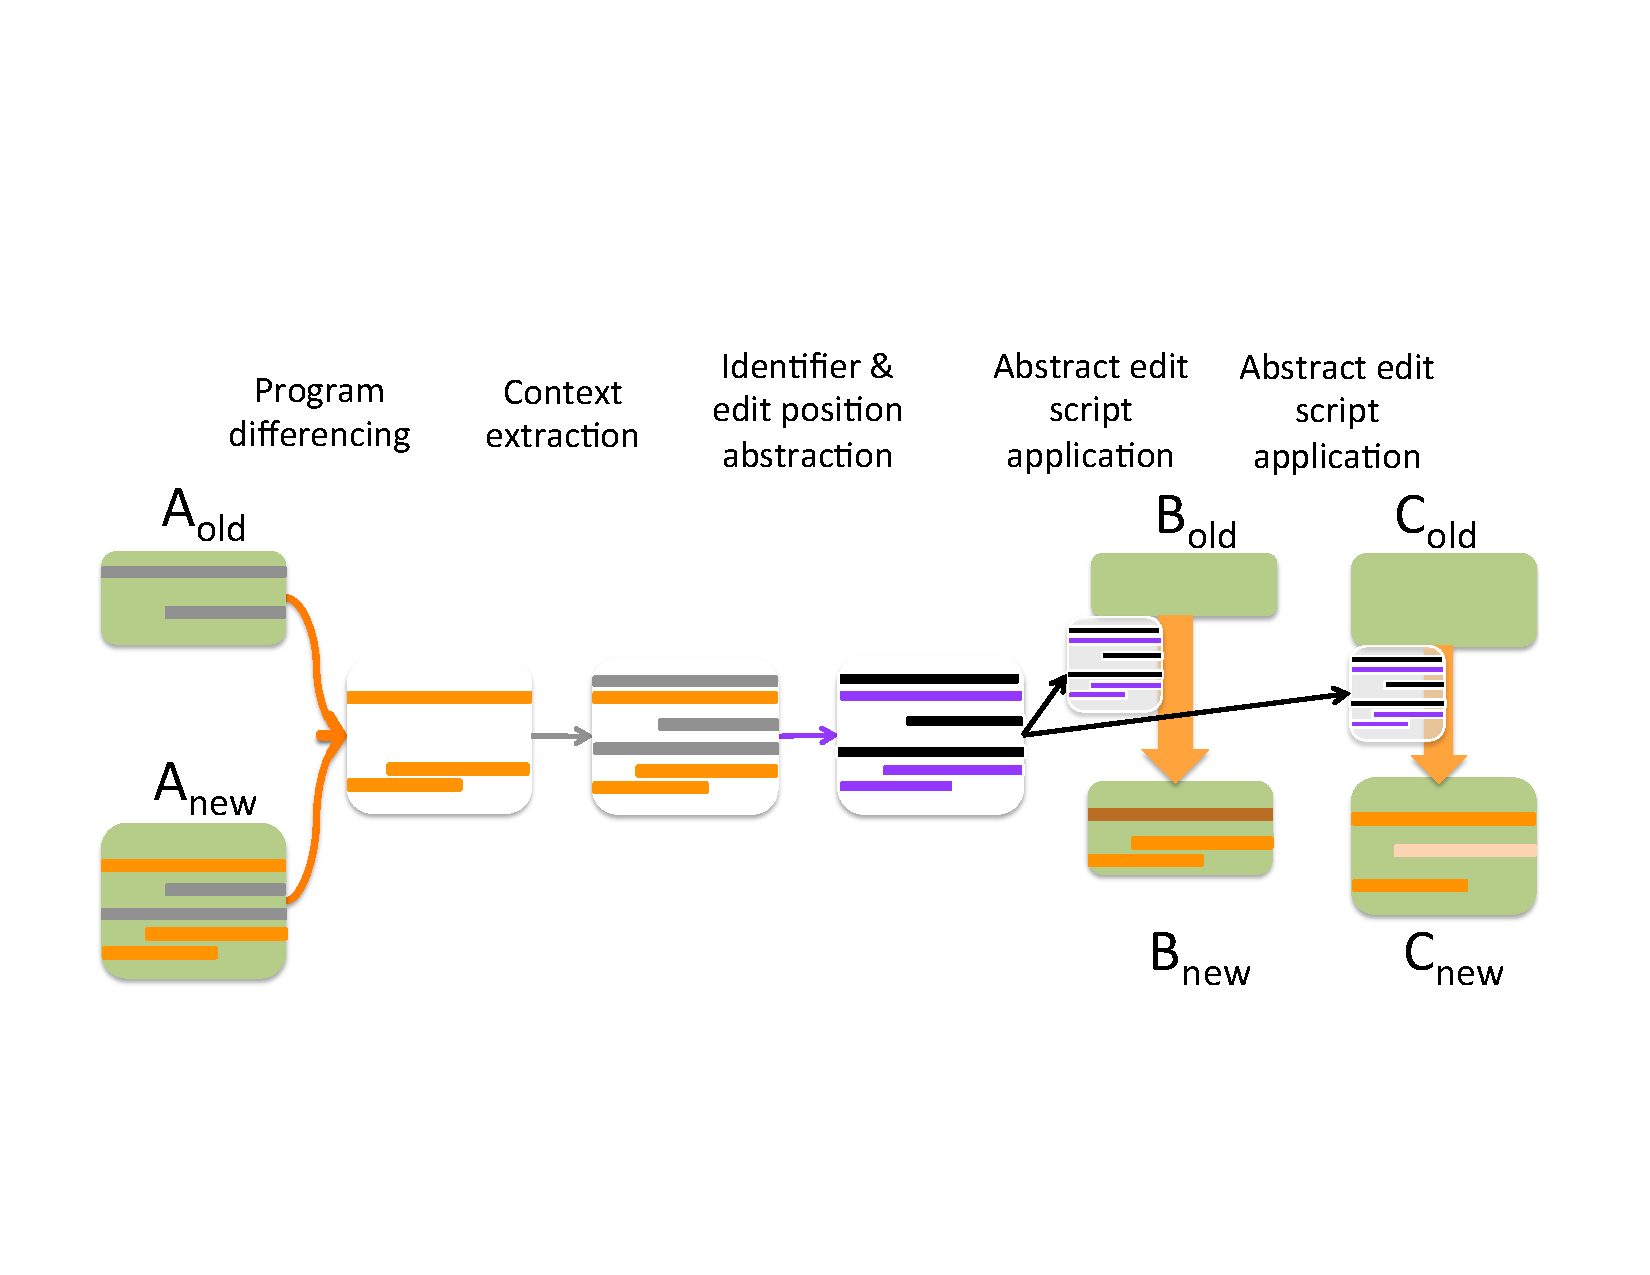
\includegraphics{images/syditoverview.pdf}}
\caption{SYDIT overview.}
\label{fig:syditoverview}
\end{figure}

As shown in Figure~\ref{fig:syditoverview}, suppose developers want to apply systematic edits to three methods: A, B, and C. Without any tool support, developers have to manually apply these similar but different edits to all three locations. With SYDIT, developers only need to (1) modify one location (e.g., A), and (2) manually specify the other locations to change (e.g., B and C). With the user input, SYDIT takes four steps to generalize and apply a program transformation. In the first step (program differencing), given the old and new version of method A, SYDIT first leverages ChangeDistiller~\cite{FWP2007} to compare the ASTs of both versions, and to extract changes as an AST edit script. The edit script may involve four types of statement-level edit operations: insert, delete, update, and move. To generalize the concrete edit script to a program transformation that is applicable to other program contexts, SYDIT needs to abstract the edit context and concrete identifiers. In step 2, SYDIT abstracts the edit context by identifying all unchanged code that is either control- or data-dependent on by the edited code, because such unchanged code manifests the semantic constraints those applied edits put on the program context. In step 3, SYDIT also abstracts the concrete identifiers used in the demonstrated edit so that the general program transformation is also applicable to code snippets that use different identifiers. Besides, SYDIT abstracts all edit operations' positions with respect to the extracted unchanged code, so that the inferred program transformation describes each edit operation within the edit-relevant context.
In this way, SYDIT derives an abstract, context-aware edit script from a given code change example.

In step 4, SYDIT concretizes the inferred program transformation to given code locations B and C, and applies the customized edits to suggest new versions of code. This step is the reverse process of the steps 1-3 mentioned above. With more details, given a code location to change (e.g., B), SYDIT first looks for any matching for the abstract edit context. If no matching is found, it indicates that similar changes should not be applied to the selected location, because the semantic constraints embedded in the abstract context are not satisfied. If one matching is found, SYDIT further concretizes the identifier usage and edit location information in the abstract script, creating a customized edit script applicable to the specific location. Finally, by modifying the code's AST based on the script, SYDIT produces a revised program for developers to review.

Although SYDIT can automate systematic editing in specified code locations, it always relies on users to manually pick those locations. In reality, finding code locations may be more challenging than applying the edits, especially when the codebase is large, and developers lack expertise of the project. Additionally, one code change example may not precisely characterize all program contexts which should be changed similarly. If the single example contains some edit-relevant context that is unique to the code location, SYDIT has no clue about how to only generalize the edit-relevant context which is commonly shared among all code locations.


\paragraph{LASE.} To facilitate systematic editing when developers cannot manually identify all code locations that should be changed similarly, LASE requires developers to provide at least two code change examples, from which it infers a general program transformation, and then leverages the transformation to both find other edit locations and suggest customized edits. 

\begin{figure}
\centering
\scalebox{0.35}{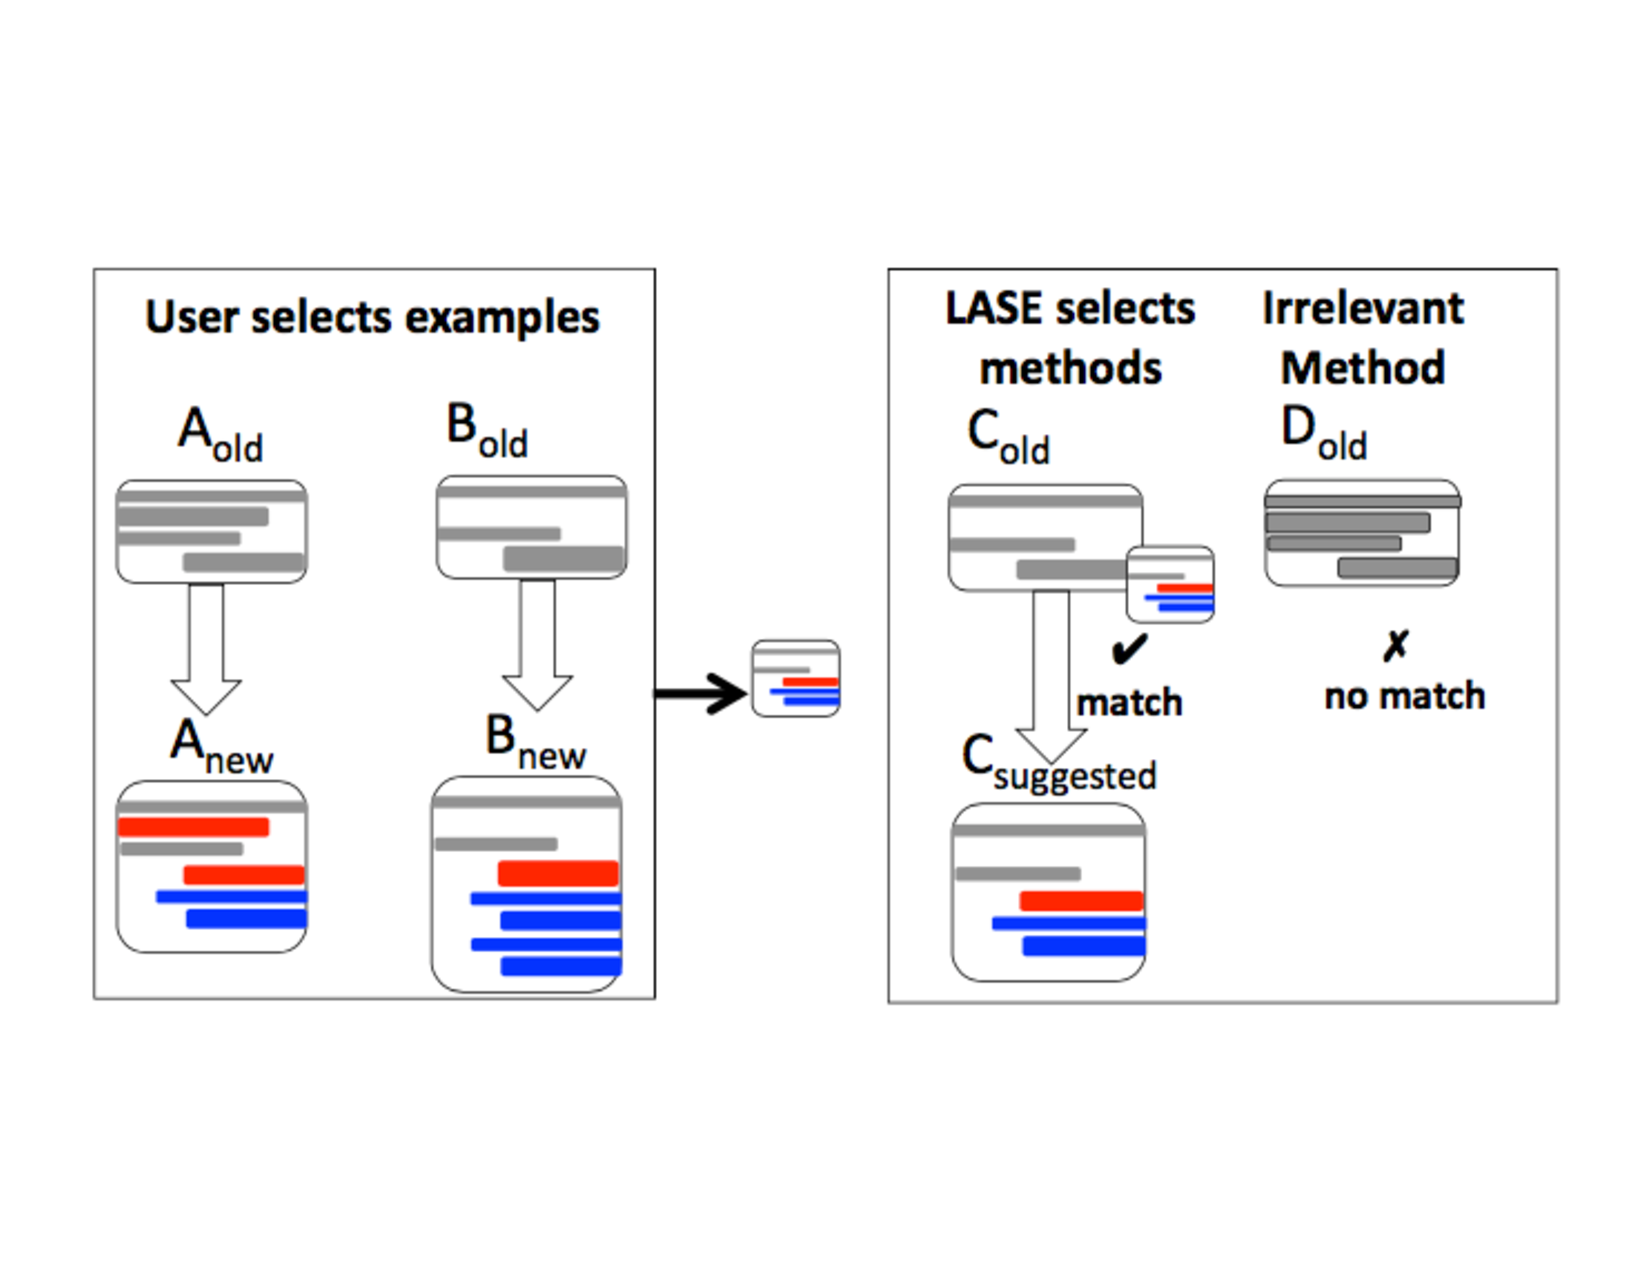
\includegraphics{images/laseoverview.pdf}}
\caption{LASE overview~\cite{MKM2013}.}
\label{fig:laseoverview}
\end{figure}

As shown in Figure~\ref{fig:laseoverview}, given two changed examples: A and B, LASE infers a general program transformation for each example, and then extracts the largest commonality between them in terms of edit operations, edit-relevant contexts, and identifier usage. In this way, LASE filters out any location-specific edit information, and only generalizes the program transformation that occurs multiple times. With such inferred program transformation, LASE attempts to establish matching between the abstract edit context and every method in the whole codebase. If a method contains a matching to the given context (e.g., C), LASE recommends the method as a candidate edit location, and suggests customized edits according to the matching information. If a method does not contain any matching to the given context (e.g., D), LASE considers the method as an irrelevant method to the systematic editing task.


\subsection{Programming by Demonstration (PbD).}
\todo{Condense PBD to 1 page or less} 
It is also called programming by example (PbE)~\cite{Lie2001}. 
This is an end-user development technique for teaching a computer or a robot new behaviors by demonstrating the task to transfer directly instead of programming it through machine commands. 

Various approaches were built to generate programs based on the text-editing actions demonstrated or text change examples provided by users~\cite{Nix1984,WiM1993,LaH1995,LWD2001}. For instance, 
TELS records editing actions, such as search-and-replace, and generalizes them into a program that transforms input to output~\cite{WiM1993}. It leverages heuristics to match actions against each other to detect any loop in the user-demonstrated program. 
Similarly, SMARTedit~\cite{LWD2001} automates repetitive text-editing tasks by learning programs to perform them using techniques drawn from machine learning. SMARTedit represents a text-editing program as a series of functions that alter the state of the text editor (i.e., the contents of the file, or the cursor position). Like macro recording systems, SMARTedit learns the program by observing a user performing her task. However, unlike macro recorders, SMARTedit examines the context in which the user's actions are performed and learns programs that work correctly in new contexts. 

Program synthesis is the task of generating a program in a domain-specific language from a given specification using some search techniques~\cite{Gul2010}. For instance, Gulwani defined a string manipulation language that supports restricted forms of regular expressions, conditionals, and loops, and also defined an algorithm to synthesize a program in this language from input-output string examples~\cite{Gul2011}. The algorithm was implemented as an interactive add-in for Microsoft Excel spreadsheet system. Each time when users manipulate a string and provide both the before- and after- versions of the manipulation, the algorithm treats the input-output example as a constraint that a desired program should satisfy, and searches for all candidate programs that can produce the output given the input. As users provide more input-output examples, the algorithm filters out the candidates that partially satisfy some of the constraints, until finding the program which satisfies all input-output constraints. Such techniques were also used in other problem domains, such as table transformation in Excel spreadsheets~\cite{HaG2011}, geometry construction~\cite{GKT2011}, data structure transformations~\cite{Feser:2015}, and hierarchical structured data manipulation~\cite{Yaghmazadeh:2016}.

\subsection{Porting programs to different languages} 
\todo{Split the following text into different languages vs. platforms} 

Developers translate code from one language to another language for various reasons. For instance, when maintaining a legacy system that was written in Fortran decades ago, programmers may migrate the system to a mainstream general purpose language, such as Java, to facilitate the maintenance of existing codebase and to extend the system by leveraging new features of the popular language. When building phone apps, Mobile developers may port a mobile application from one platform (e.g., Android) to another (e.g. iOS) by translating code from Java to Swift. 

Most researchers and engineers built cross-language program transformation tools by hard coding the translation rules and implementing any missing equivalent functionality between languages~\cite{Yasumatsu:95,Mossienko:03,Sneed:2010,jovial2c,cobol2java}. For instance, SPiCE translates Smalltalk programs to C~\cite{Yasumatsu:95}. The two languages are different in two aspects. First, the execution model of Smalltalk, which creates activation records as objects, is very different from that of C. Second, Smalltalk and C have very different approaches to storage management. To overcome the challenges, Yasumatsu et al.~created runtime replacement classes implementing the same functionality of Smalltalk classes that are inherently part of the Smalltalk execution model. They also provided semi-conservative real-time compacting garbage collection that works without language support.
Mossienko~\cite{Mossienko:03} and Sneed~\cite{Sneed:2010} automated COBOL-to-Java code migration by defining and implementing rules to generate Java classes, methods, and packages from COBOL programs. Although some of these tools can perform very complicated code translations tasks, it always costs a lot of time and effort to manually build such tools from scratch between any two languages. HTML5 is a markup language used for structuring and presenting content on the World Wide Web~\cite{html5}. To simplify cross-platform mobile software development, PhoneGap~\cite{phonegap} was built to automatically translate HTML5 implementation to Android or iOS native code.

\subsection{Porting programs to different platforms} 

\section{An Organized Tour of Seminal Papers: II. Inspecting Program Changes}

\subsection{Code Reviews Practices}
since code reviews is a common context where change inspection happens ( peter rigby)  code flow, collaborators in industry. generally starting from code review practices

\todo{Miryung to Tianyi: make the introduciton a little bit broad} 
Peer code review is a quality assurance mechanism that requires software developers to manually inspect each other's source code to find programming mistakes overlooked in the initial development phase. In 1976, Fagan formalized code review as a highly structured inspection process with multiple stages (e.g., {\em overview}, {\em preparation}, {\em inspection}, {\em rework}, {\em follow-up}) and multiple participants (e.g., {\em moderator}, {\em designer}, {\em implementor}, and {\em tester})~\cite{fagan2001design}. This inspection process is performed at the end of each software development phase (e.g., design, implementing, testing), in which software developers attend a series of group meetings and review design documentations and source code line by line. Such careful and thorough inspection process has been proven effective in terms of finding bugs, but the cumbersome and time-consuming nature of this process hinders its universal adoption in practice. 


\begin{figure}[ht]
 \centering
 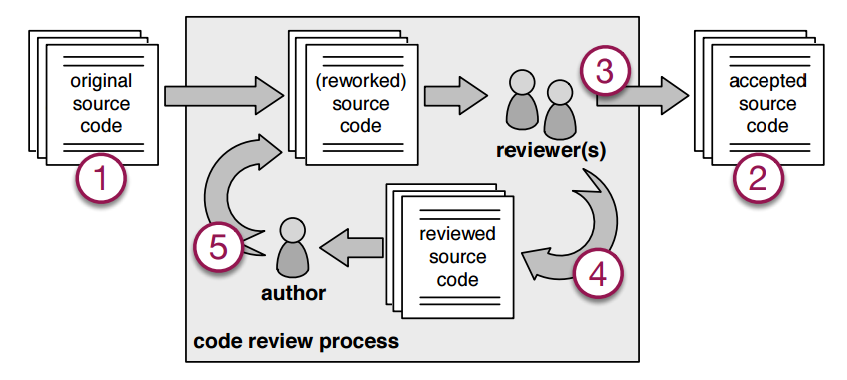
\includegraphics[width=0.8\textwidth]{images/review-process.png}
 \caption{The modern code review process (based on~\cite{beller2014modern})}
 \label{fig:review-process}
\end{figure}

Nowadays many organizations adopt lightweight code review processes with less overhead than formal code inspections. In contrast to formal code review, modern code review occurs more regularly (often on a daily basis) and does not require a dedicated code review team with particular members. In particular, there is a clear trend towards utilizing code review tools to support code review tasks, instead of organizing and attending group meetings. Figure~\ref{fig:review-process} shows the overall process of a code review task. The {\em author} first submits the {\em original source code} for review. The {\em reviewers} then decide whether the submitted code meets the project's quality acceptance criteria. If not, reviewers can add review comments to the source code and send the {\em reviewed source code} back to the author. The author then revises the source code to address reviewers' comments and then send it back for further review. This process continues till all reviewers accept the revised source code. Modern code review is widely practiced both in open-source and industrial contexts and is recognized as a valuable tool to remove common vulnerabilities, performance bugs, and style issues. 


\todo{Tianyi: Could you please expand upon the following a little more. I would like this to be about 2 pages in total with some references to recent work such as a short 4 page paper by MSR on code reviews in ICSE 2016.}  
Recent studies have investigated the common practices and challenges in modern code review. Rigby et al.~conduct a case study in an open-source software project, Apache HTTP server, using archived code review records in email discussions and version control repositories~\cite{rigby2008open}. They find that, in contrast to traditional software inspection (Fagan style), modern code review in open-source projects often involves frequent review tasks of small yet complete program contributions, conducted asynchronously by a small group of self-selected experts. Rigby and Bird conduct a similar investigation on a more diverse set of software projects, including two two Google-led projects, Android and Chromium OS, three Microsoft projects, Bing, Office, and MS SQL, and internal projects at Advanced Micro Devices (AMD)~\cite{rigby2013convergent}. They find several convergent code review practices that may indicate general principles of modern code review. For example, modern code review often involves two reviewers and is performed regularly and quickly. They also observe the benefits of sharing knowledge across the development team via peer code review. In order to understand the expectations, outcomes, and challenges of modern code review, Bacchelli and Bird observe, interview, and survey software developers at Microsoft and manually classify hundreds of review comments across several Microsoft teams~\cite{bacchelli2013expectations}. They find that, although the top motivation of code review is finding defects, the actual outcomes are less about finding defects than expected: only a small portion of review comments are related to software defects, which mainly cover small, low-level logical issues. A key challenge reported by reviewers is the lack of tool support for code change comprehension during peer code review. Tao et al.~also study the challenges that developers face when they comprehend code changes and find that modern code review tools must support the capability to divide a large chunk of code changes into small, cohesive groups and to filter non-essential changes~\cite{tao2012software}. 

\todo{The following text should be placed under code review practices}. 

Prior work also observes that developers often submit program changes from multiple programming tasks (e.g., bug fixing, refactorings, feature additions) to a single code review. Reviewers sometimes use ``chunky changes'' or ``code bombs'' to describe such large, unrelated changes that are bundled in a single review. Such changes often lead to difficulty in change comprehension, since reviewers have to mentally ``untangle'' them to figure out which subset of changes addresses which issue first~\cite{kawrykow2011non, murphy2012we, herzig2013impact}. Reviewers have indicated that they can better understand small, cohesive changes rather than large, tangled ones~\cite{rigby2008open}. For example, a code reviewer commented on Gson revision 1154 saying ``I would have preferred to have two different commits: one for adding the new {\ttt getFieldNamingPolicy} method, and another for allowing overriding of primitives.''\footnote{\url{https://code.google.com/p/google-gson/source/detail?r=1154}} This motivates the need of decoupling composite changes in a large code review. 


\subsection{Techniques for Code Change Comprehension} 
\todo{Tianyi: Make one of the commercial code review tools a little bit more concrete and go deeper with screen shots. the following text seems like it was just copied from the intro of critics paper.}

Code review is effective only when reviewers are able to understand the changes being made. When the information required to inspect code changes is distributed across multiple files, developers find it difficult to inspect code changes~\cite{dunsmore2000object}. For example, when an API gets modified in the latest release, all call sites using this API must be updated correctly. Such edits tend to be systematic\textemdash involving similar but not identical edits to multiple locations.


\todo{For example, take a snapshot of CodeFlow or Code Collaborator, describe the tool's feature in more detail. target length should be 1 page including a screenshot.}  

Unfortunately, popular code review tools\textemdash Facebook's {\phabricator},\footnote{\url{http://phabricator.org}} Google's {\gerrit},\footnote{\url{http://code.google.com/p/gerrit/}} and Microsoft's {\codeflow},\footnote{\url{http://visualstudioextensions.vlasovstudio.com/2012/01/06/codeflow-code-review-tool-for-visual-studio/}}\textemdash all compute program differences per file. This obliges reviewers to read changed lines file by file, even when those cross-file changes are done systematically to address the same issue. Therefore, reviewers are left to manually inspect individual edits to answer questions such as ``what other code locations are changed similar to this change?'' and ``are there any other locations that are similar to this code but are not updated?''


\subsubsection{Interactive Code Review using Code Patterns} 
\todo{Right now there's too much focus on Critics. Reduce the length to be 1.5 pages including a screen snapshot.}
\begin{figure}[ht]
 \centering
 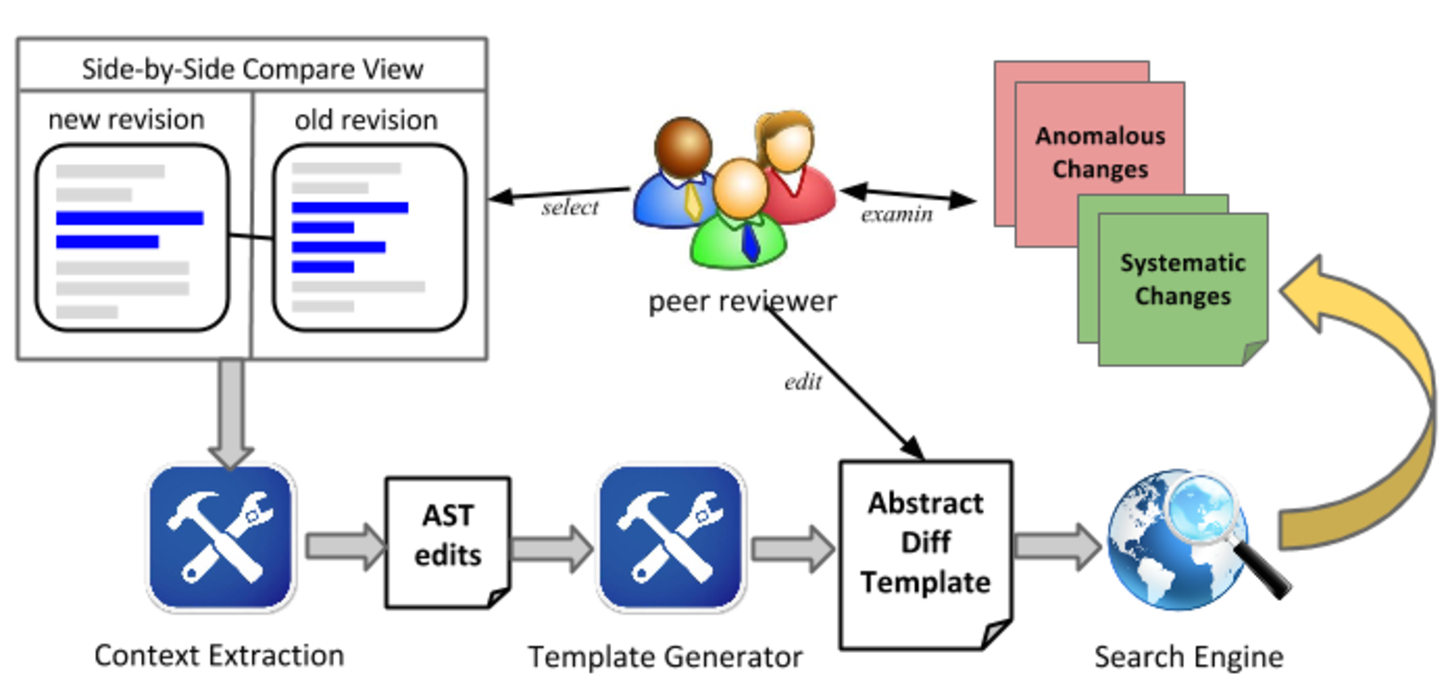
\includegraphics[width=0.8\textwidth]{images/critics-workflow.pdf}
 \caption{The workflow of {\critics}}
 \label{fig:critics-workflow}
\end{figure}

To address this issue, Zhang et al.~present {\critics}, a novel approach that allows reviewers to interactively inspect such systematic changes during peer code review~\cite{zhang2015interactive}. Figure~\ref{fig:critics-workflow} describes the interactive workflow of {\critics}. Given a specified change that a reviewer would like to inspect, {\critics} creates a change template from the selected change, which serves as the pattern for searching similar changes. {\critics} includes {\em change context} in the template---unchanged, surrounding program statements that are relevant to the selected change. {\critics} models the template as Abstract Syntax Tree (AST) edits and allows reviewers to iteratively customize the template by parameterizing its content and by excluding certain statements. {\critics} then matches the customized template against the rest of the codebase to summarize similar changes and locate potential inconsistent or missing changes. Reviewers can incrementally refine the template and progressively search for similar changes until they are satisfied with the inspection results. This interactive feature allows reviewers with little knowledge of a codebase to flexibly explore the program changes with a desired pattern.



\begin{figure}[ht]
 \centering
 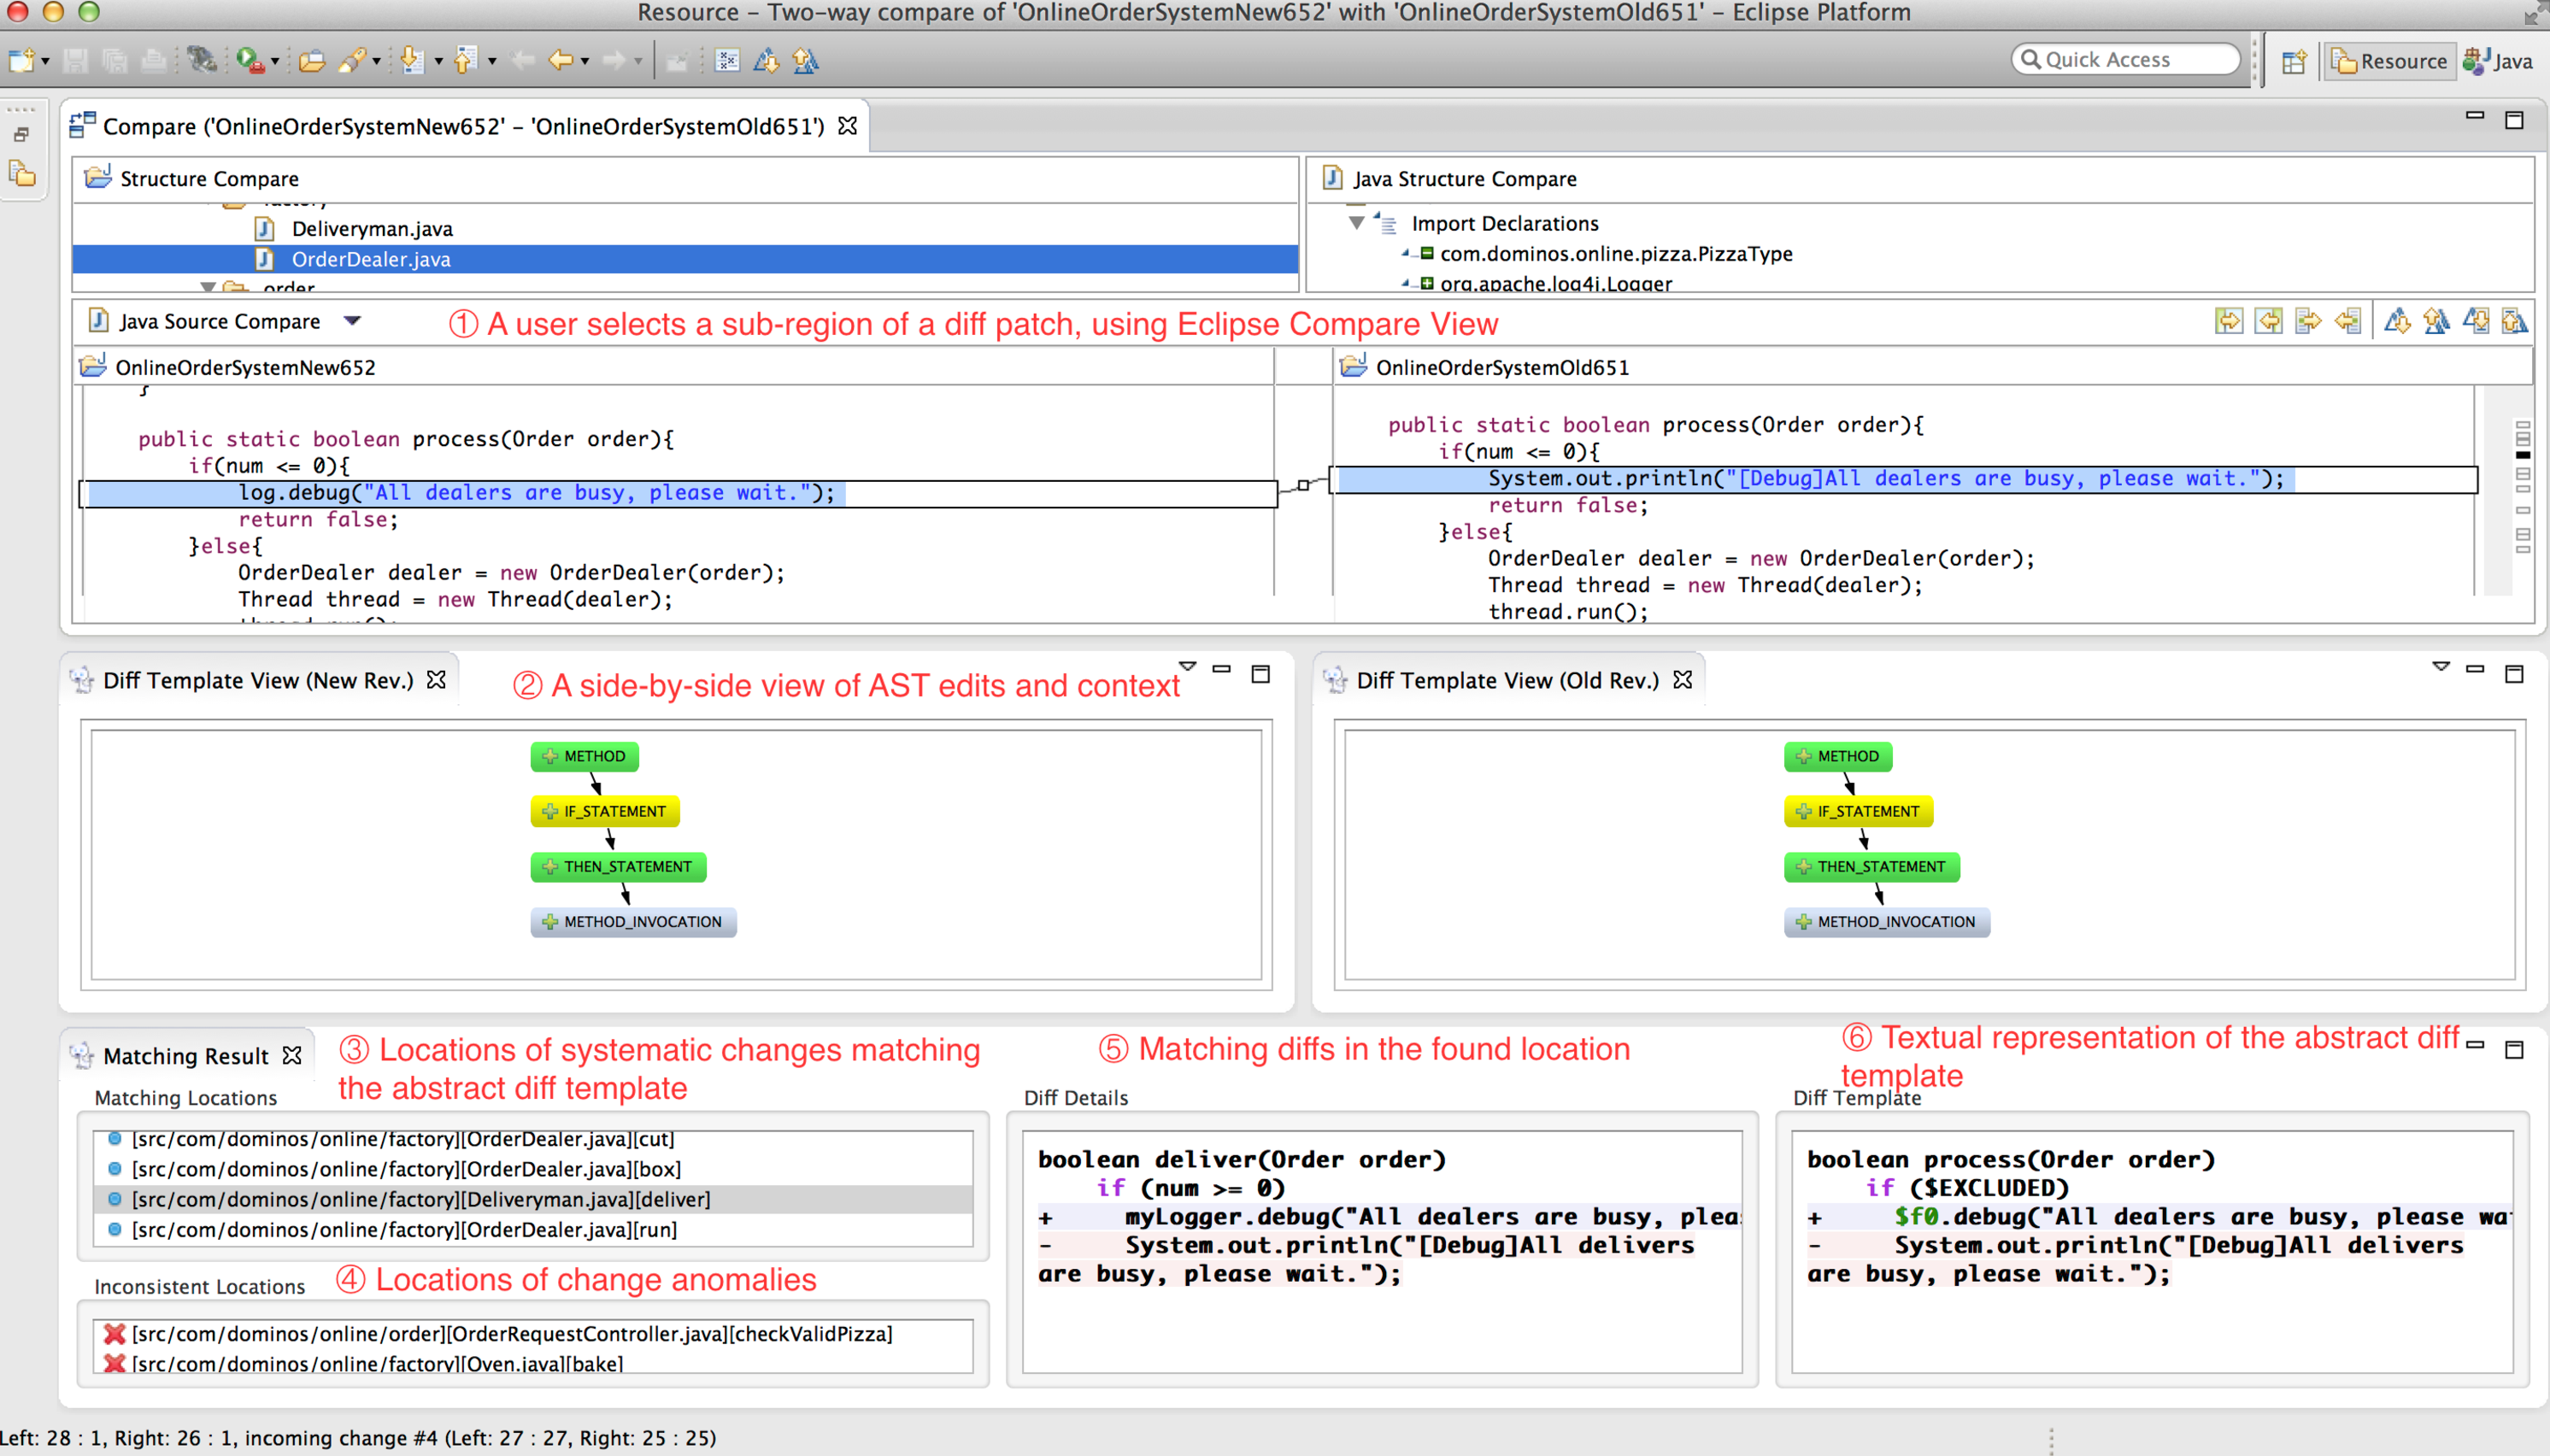
\includegraphics[width=\textwidth]{images/critics-UI.pdf}
 \caption{A screen snapshot of {\critics}'s Eclipse plugin and its features}
 \label{fig:critics-UI}
\end{figure}

{\critics} is implemented as an Eclipse plugin.\footnote{{\critics}'s tool and evaluation dataset are available online \url{https://sites.google.com/a/utexas.edu/critics/}} Figure~\ref{fig:critics-UI} shows a screenshot of {\critics} plugin. {\critics} is integrated with the {\bf Compare View} in Eclipse, which displays line-level differences per file (see \ding{172} in Figure~\ref{fig:critics-UI}). A user can specify a program change she wants to inspect by selecting the corresponding code region in the Eclipse Compare View. The {\bf Diff Template View} (see \ding{173} in Figure~\ref{fig:critics-UI}) visualizes the change template of the selected change in a side-by-side view. Reviewers can parameterize concrete identifiers and exclude certain program statements by clicking on the corresponding node in the Diff Template View. {\bf Textual Diff Template View} (see \ding{177} in Figure~\ref{fig:critics-UI}) shows the change template in a unified format. The {\bf Matching Result View} summarizes the consistent changes as {\em similar changes} (see \ding{174} in Figure~\ref{fig:critics-UI}) and inconsistent ones as {\em anomalies} (see \ding{175} in Figure~\ref{fig:critics-UI}).

\todo{the evaluation and quotes are too much for this chapter. so I removed them} 

\subsubsection{Change Decomposition} 

To address this issue, Barnett et al.~present {\clusterchanges}, a lightweight static analysis technique for decomposing large changes. The insight is that program changes that address the same issue can be related via implicit dependency information such as {\em def-use} relationship. For example, if a method definition is changed in one location and its callsites are changed in two other locations, these three changes are likely to be related and should be reviewed together. Given a code review task, {\clusterchanges} first collects the set of definitions for types, fields, methods, and local variables in the corresponding project under review. Then {\clusterchanges} scans the project for all uses (i.e., references to a definition) of the defined code elements. For instance, any occurrence of a type, field, or method either inside a method or a field initialization is considered to be a use. Based on the extracted def-use information, {\clusterchanges} identifies three relationships between program changes. 

\todo{Remove a bullet list and integrate into text.}
\begin{itemize}
 \item {\bf Def-use relation}. If the definition of a method or a class field is changed, all the uses should also be updated. The change in the definition and the corresponding changes in its references are considered related.
 \item {\bf Use-use relation}. If two or more uses of a method or a class field defined within the change-set are changed, these changes are considered related. 
 \item {\bf Enclosing relation}. Program changes in the same method are considered related because a) based on observation, program changes to the same method are often related, (b) reviewers often inspect methods atomically rather than reviewing different changed regions in the same method separately.
\end{itemize}

Given these relations, {\clusterchanges} creates a partition over the set of program changes by computing a transitive closure of related changes. On the other hand, if a change is not related to any other changes, it will be put into a specific partition, {\em miscellaneous changes}.

\todo{Expand the following technique a little bit more. Give similar weights to ClusterChange.}
Independently from {\clusterchanges}, Tao et al.~present a similar change decomposition technique that leverages more sophisticated heuristics, other than the def-use analysis only~\cite{tao2015partitioning}. Tao et al.~cluster changes based on the following heuristics.


\subsection{Program Differencing} 
program differencing (going to back history of differencing, diff, AST diff, CFG diff, PDG diff.--- mention its symmetric problem of clone detection)
go deeper for a few techniques that help with change comprehension: kim et al. critics, chris bird at MS


\section{An Organized Tour of Seminal Papers: III. Debugging and Testing Program Changes} 

\subsection{Delta Debugging: Finding Code Changes Causing Errors}
\todo{2 pages} 
\subsection{Regression Testing} 
\todo{2 pages} 
\paragraph{Change Impact Analysis} 
\todo{2 pages} 

\section{Future Directions and Open Problems} 
\todo {4 pages} 


\subsubsection*{Acknowledgments.} The heading should be treated as a
subsubsection heading and should not be assigned a number.

\section{The References Section}\label{references}
\bibliography{tianyi,mengna}
\bibliographystyle{abbrv}

\section*{Appendix} 
\end{document}
